\bchapter{PyTorch Mobile}
\section{PyTorch \& PyTorch Mobile}
PyTorch\cite{Pytorch} è un framework di deep learning open source, sviluppato inizialmente da \textit{Meta AI} e ora parte della \textit{Linux Foundation}.
Progettato con Python, viene usato per creare reti neurali e per progetti di apprendimento automatico,
combinando la libreria di machine learning \textbf{Torch}\cite{Torch} con un’API di alto livello basata su Python. Torch è famosa, specialmente nel campo
del Deep Learning, per fornire tool semplici e flessibili insieme a performance elevate; uno dei sui punti salienti è il grande supporto per le GPU, che 
contribuisce ad un allenamento più efficiente dei modelli di deep learning.
PyTorch fornisce innanzitutto un pacchetto Python per funzionalità ad alto livello, come l'elaborazione dei \textbf{tensori}\footnote{Array multidimensionale utilizzato per memorizzare dati. Nel campo del Machine Learning vengono usati per rappresentare e manipolare input, pesi e output.}
ed inoltre un così detto \textbf{TorchScript}, che permette di creare modelli da PyTorch che possono poi venire salvati e caricati in un processo dove non c'è alcuna 
dipendenza di Python.

PyTorch Mobile\cite{PyTorchMed}, introdotto per la prima volta nel 2019 alla \textit{PyTorch Developer Conference}, si riferisce ad un set di librerie e funzionalità fornite da PyTorch che
permettono allo sviluppatore di eseguire un modello PyTorch direttamente su dispositivi mobili, come smartphone e tablet.

\section{Caratteristiche Principali}
Le caratteristiche principali di PyTorch, così come scritto sul sito ufficiale\cite{PyTorchOfficial}, sono:
\begin{itemize}
    \item Disponibile per iOS, Android e Linux;
    \item Fornisce API per comuni compiti di pre-processing e integrazione necessari ad incorporare Machine Learning nelle applicazioni mobile;
    \item Supporta la libreria XNNPACK per le CPU Arm e integra QNNPACK per i kernel a 8 bit quantizzati;
    \item Fornisce un efficiente interprete mobile per Android e iOS;
    \item Supporterà a breve backend hardware come GPU, DSP e NPU.
\end{itemize}

XNNPACK\cite{XNNPACK} è una libreria altamente ottimizzata per accelerare le operazioni di reti neurali convoluzionali (CNN) e altre operazioni di reti neurali su hardware mobile,
mentre QNNPACK\cite{QNNPACK} (Quantized Neural Network PACKage) è progettata per accelerare le reti neurali quantizzate\footnote{La quantizzazione è un processo che riduce la precisione dei numeri usati nei calcoli di una rete neurale, da 32-bit a 8-bit o meno, riducendo così l'uso della memoria e migliorando le prestazioni senza sacrificare significativamente l'accuratezza.}
su hardware mobile.


\section{Da un modello PyTorch a PyTorch Mobile}
Il tipico flusso dalla creazione del modello in PyTorch all'implementazione sul dispositivo mobile può essere visionato in figura \ref{fig:pyworkflow}; di seguito
verranno spiegati i vari step.

\begin{figure}[ht]
    \centering
    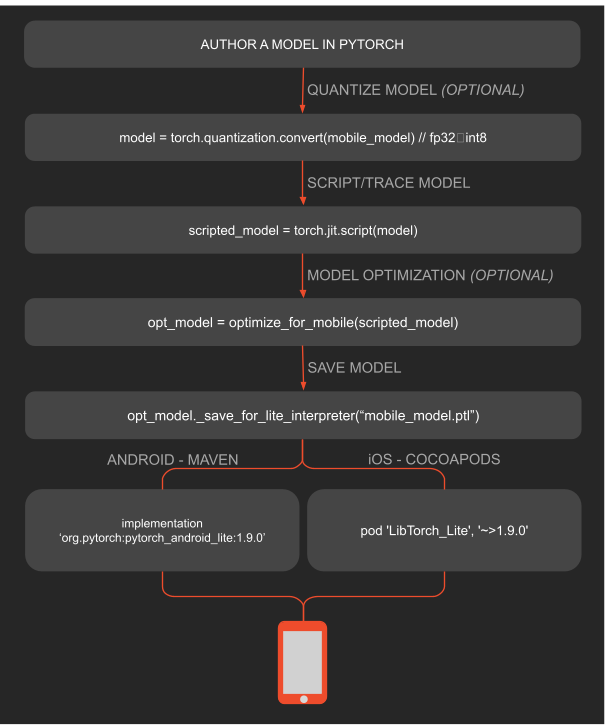
\includegraphics[width=0.5\textwidth]{Immagini/workflow_pytorch.png}
    \caption{Workflow dal training al rilascio di un modello su piattaforma mobile. Fonte \cite{PyTorchOfficial}}
    \label{fig:pyworkflow}
\end{figure}

\subsection{Costruire un modello in PyTorch}
\subsection{Quantizzazione}
\subsection{Scripting e Tracing del modello}
\subsection{Ottimizzazione}
%\subsection{Salvataggio}
